\documentclass[12pt]{article}
\usepackage{amssymb,mathtools, systeme}
\usepackage[margin=1in]{geometry}
\usepackage{fancyhdr}
\usepackage{circuitikz}
\usepackage{graphicx}
\graphicspath{ {./Figures/} }
\usepackage{amsmath}
\usepackage{ragged2e}
\usepackage{subcaption} 
\usepackage{float}
\usepackage{cancel}
\usepackage{siunitx}
\pagestyle{fancy}
\usepackage[shortlabels]{enumitem}
\usepackage{mathtools}
\makeatletter
\renewcommand*\env@matrix[1][\arraystretch]{%
  \edef\arraystretch{#1}%
  \hskip -\arraycolsep
  \let\@ifnextchar\new@ifnextchar
  \array{*\c@MaxMatrixCols c}}
\makeatother
\newcommand*{\permcomb}[4][0mu]{{{}^{#3}\mkern#1#2_{#4}}}
\newcommand*{\Comb}[2]{{}^{#1}C_{#2}}%
\DeclarePairedDelimiter\ceil{\lceil}{\rceil}
\DeclarePairedDelimiter\floor{\lfloor}{\rfloor}
\setlength{\headheight}{15 pt}
\lhead{Georgy Antonov}
\chead{HW 7}
\rhead{Neural Dynamics}

\begin{document}\noindent


\noindent\textbf{Question 1. Nonlinear network with two divisive inhibitory neurons.}
\begin{enumerate}
\item[1.1] We have a network of two nonlinear neurons with divisive feedback given by the following system of differential equations
\begin{align*}
    \tau \dot{u}_{1}(t) &= -u_{1}(t) + \frac{s_{1}}{1+u_{2}(t)}\\
    \tau \dot{u}_{2}(t) &= -u_{2}(t) + \frac{s_{2}}{1+u_{1}(t)}
\end{align*}
where $s_{1}$ and $s_{2}$ are two nonnegative inputs, respectively. We are required to prove that 
when the initial condition $\mathbf{u}(\mathbf{0})$ lies in the first quadrant of the state space with $u_{1}$, $u_{2} \geq 0$, the system stays in the first quadrant forever.
\begin{figure}[h!]
    \centering
    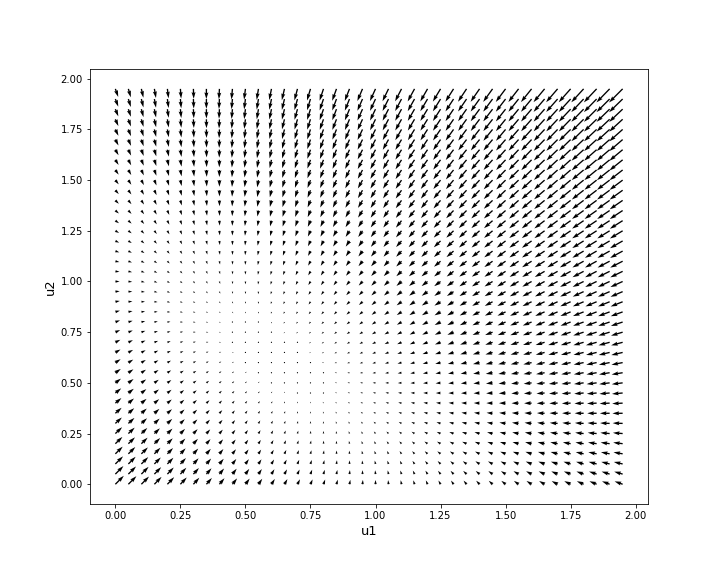
\includegraphics[width=1\textwidth]{./fig1.png}
    \caption{Vector field dynamics for the given nonlinear dynamical system for $u_{1}, u_{2} \geq 0$.}
\end{figure}\\
\noindent The dynamics of the vector field for $s_{1}=1$, $s_{2}=1$, and $\tau = 1 \, \text{ms}$ appears in Figure 1.
Note that in order for the system to stay in the first quadrant, whenever $u_{1}$ or $u_{2}$ is at the boundary, its derivative has to be nonnegative.
Thus, we have
\[
    u_{1}=0 \implies \frac{du_{1}}{dt} \geq 0 \Leftrightarrow u_{2} > -1
\]
\[
    u_{2}=0 \implies \frac{du_{2}}{dt} \geq 0 \Leftrightarrow u_{1} > -1
\]
\item[1.2] To compute the fixed points for an input of the form $s_{1} = s_{2} \geq 0$, we can plot the isoclines
\begin{align*}
    \frac{du_{1}}{dt} = 0 \implies u_{1}=\frac{s_{1}}{1+u_{2}}\\
    \frac{du_{2}}{dt} = 0 \implies u_{2}=\frac{s_{2}}{1+u_{1}}
\end{align*}
A stationary point is then given by the intersection of these two isoclines
\[
    u_{1} = \frac{s_{1}(1 + u_{1})}{1 + u_{1} + s_{2}} \, \Leftrightarrow  \, u_{1}^2 + u_{1}(s_{2} - s_{1} + 1) - s_{1} = 0
\]
Since we are given that $s_{1}=s_{2}$, this simplifies to
\[
    u_{1}^2 + u_{1} - s_{1} = 0
\]
And we therefore find that
\begin{align*}
    u_{1} &= \frac{-1 + \sqrt{1 + 4s_{1}}}{2}\\
    u_{2} &= \frac{2s_{2}}{1 + \sqrt{1 + 4s_{1}}}  
\end{align*}
The two isoclines are plotted in Figure 2.
\begin{figure}[h!]
    \centering
    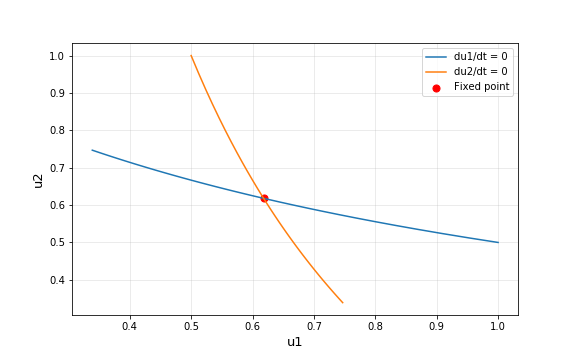
\includegraphics[width=1\textwidth]{./fig2.png}
    \caption{Computed fixed point given by the intersection of the two isoclines for $s_{1}=s_{2}=1$.}
\end{figure}\\
For $s_{1}=s_{2}=0$ the fixed point appears at $u_{1}=u_{2}=0$ and for $s_{1}=s_{2}=3/4$ it is at $u_{1}=u_{2}=0.5$.
\item[1.3]


Recall that for the system 
\[
    \dot{\mathbf{x}} = \mathbf{f}(\mathbf{x}(t))
\]
points with $\mathbf{f}(\mathbf{x})=\mathbf{0}$ are called fixed points, for the dynamics at these points does not change. Also recall that the linear dynamical system
\[
    \dot{\mathbf{u}}(t) = \mathbf{A}\mathbf{u}(t)
\]
where 
\[
    \mathbf{A} = \frac{\partial{\mathbf{f}(\mathbf{u}_{0})}}{\partial{\mathbf{u}}}
\]
is called the linearised dynamics at the point $\mathbf{u}_{0}$. For the system given, the linearised dynamics at $\mathbf{u}_0$ is of the form
\[
\mathbf{A} = \frac{\partial{\mathbf{f}}}{\partial{\mathbf{u}}}\bigg|_{\mathbf{u}_0} = \frac{1}{\tau}\begin{pmatrix}[1.5] -1& -\frac{s_{1}}{(1+u_{0,2})^2}\\ -\frac{s_{2}}{(1 + u_{0,1})^2}& -1\end{pmatrix}
\]
After eigendecomposition, the eigenvectors of the linearised dynamics matrix are
\[
    v_{1}=\begin{pmatrix}1\\ 1\end{pmatrix}, \, v_{2}=\begin{pmatrix}-1\\ 1\end{pmatrix}
\]
and the corresponding eigenvalues are
\begin{align*}
    \lambda_{1} &= \frac{-s \tau - u_{0}^2-2u_{0}-1}{\tau^2(u_{0}+1)^2}\\
    \lambda_{2} &= \frac{s \tau - u_{0}^2-2u_{0}-1}{\tau^2(u_{0}+1)^2}
\end{align*}
where $s=s_{1}=s_{2}$ and $u_{0}=u_{0,1}=u_{0,2}$.
To analyse the stability of the system we need to fix $\tau$ and consider inputs of varying strength. For example, consider $\tau = 1 \, \text{ms}$ and $s=1$. Then the fixed point
coordinates are $u_{0}=0.618$ and the linearised dynamics matrix is
\[
\mathbf{A} = \begin{pmatrix}[1.5] -1 & -0.381966\\ -0.381966 & -1\end{pmatrix}  
\]
The eigenvlues for this dynamics are
\[
    \lambda_{1}=\frac{-2-\sqrt{0.58359}}{2}=-1.38196, \, \lambda_{2}=\frac{-2+\sqrt{0.58359}}{2}=-0.6180
\]
Both of the eigenvalues are negative, and hence the fixed point is stable.
\item[1.4] Phase portraits for two different inputs appear in Figures 3 \& 4.
\begin{figure}[h!]
    \centering
    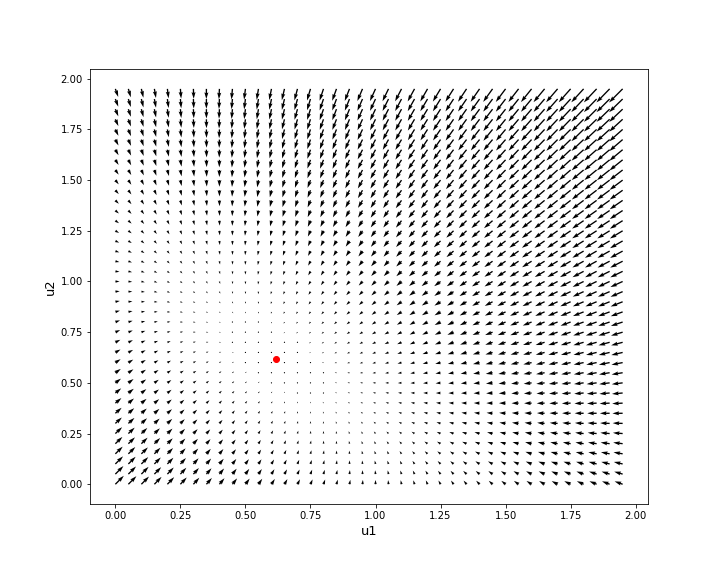
\includegraphics[width=1\textwidth]{./fig3.png}
    \caption{Phase portrait for $s=1$. The fixed point is shown in red.}
\end{figure} 
\begin{figure}[h!]
    \centering
    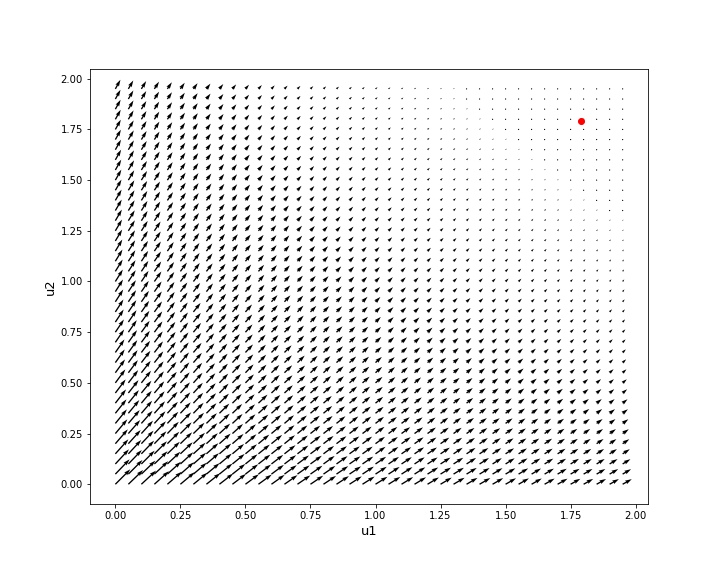
\includegraphics[width=1\textwidth]{./fig4.png}
    \caption{Phase portrait for $s=5$. The fixed point is shown in red.}
\end{figure} 
\item[1.5] We are required to derive a Lyapunov function for the given system. Let us denote
\[
    F(u_{1}, u_{2})=  \frac{1}{\tau}\left(-u_{1} + \frac{s_{1}}{1+u_{2}}\right)
\] 
\[
    G(u_{1}, u_{2})=   \frac{1}{\tau}\left(-u_{2} + \frac{s_{2}}{1+u_{1}}\right)
\]
Then, since both $F$ and $G$ are $C^1$ and have a finite number of joint zeroes, then by the Lyapunov theorem the following function with $|\epsilon| < 1$
\[
    E(\mathbf{u}) = \frac{1}{2}F^2(\mathbf{u}) + \epsilon F(\mathbf{u})G(\mathbf{u}) + \frac{1}{2}G^2(\mathbf{u})
\]
is positive definite in regions around each zero. The resulting Lyapunov function for $|\epsilon| = 0$ is
\begin{align*}
    E(u_{1}, u_{2})&=\frac{1}{2}F^2(u_{1}, u_{2}) + \frac{1}{2}G^2(u_{1}, u_{2}) \\
    &= \frac{1}{2\tau}\left( \left(-u_{1} + \frac{s_{1}}{1+u_{2}}\right)^2 + \left(-u_{2} + \frac{s_{2}}{1+u_{1}}\right)^2 \right)
\end{align*}
The derivative of Lyapunov function is of the form
\[
    \dot E(u_{1}, u_{2}) = F^{2}\frac{\partial F}{\partial u_{1}} + FG\left(\frac{\partial F}{\partial u_{2}} + \frac{\partial G}{\partial u_{1}}\right) + G^{2}\frac{\partial G}{\partial u_{2}}
\]
Hence, if we let $a=c=\frac{\partial F}{\partial u_{1}}=\frac{\partial G}{\partial u_{2}}=-\frac{1}{\tau}$ then, if the derivative $\dot E(u_{0}, u_{1})$ is negative definite in 
the regions surrounding the fixed points, then the function $E(\mathbf{u})$ is truly Lyapunov. Thus, we check the corollary condition
\[
    |b|=\bigg|\frac{\partial F}{\partial u_{2}} + \frac{\partial G}{\partial u_{1}}\bigg| = \frac{1}{\tau}\bigg|-\frac{s}{(1+u_{2})^2} -\frac{s}{(1+u_{1})^2}\bigg|<\frac{2}{\tau}
\]
which simplifies to
\[
    \frac{s}{(1+u_{2})^2} +\frac{s}{(1+u_{1})^2}<2
\]
The condition is fulfilled when
\begin{align*}
    (1+u_{0})^2 &> s\\
    \implies 1 + 2u_{0} + u_{0}^{2} &> s\\
    \implies u_{0}^{2} + 2u_{0} + (1-s) &> 0
\end{align*}
where $u_{0}=u_{1}=u_{2}$. Therefore, we have
\[
    u_{0}=\frac{-2 \pm \sqrt{3-s}}{2}
\]
For $s=3/4$, we find
\[
      u_{0}=-1.75; \, -0.25 
\]
Thus, the function is Lyapunov for $s=3/4$ when $u_{0} \in (-0.25, +\infty)$.\\
\\
Also observe that the left hand side of the condition is at maximum when $u_{1}=u_{2}=0$. Hence, for the condition to be fulfilled, we require $s<1$.
\end{enumerate}
\newpage
\noindent\textbf{Question 2. Simple autoassociative memory.}
\begin{enumerate}
\item[2.1] Assume an autoassociative memory network given by
\[
    \tau \mathbf{\dot u}(t) = -\mathbf{u}(t) + [\mathbf{Mu}(t)]_{+}
\]  
where matrix $\mathbf{M}$ is 
\[
\mathbf{M}=\begin{pmatrix}1 & -0.1 & -0.1\\ -0.1 & 1 & -0.1\\ -0.1 & -0.1 & 1\end{pmatrix}  
\]
We are required to find an equation which determines the stationary points of the network. Similarly to Question 1, 
the stationary points are described by the intersections of isoclines. Therefore, we solve
\begin{align*}
    \frac{du_{1}}{dt} &= 0 \implies u_{1}=[u_{1} -0.1u_{2}-0.1u_{3}]_{+}\\
    \frac{du_{2}}{dt} &= 0 \implies u_{2}=[-0.1u_{1} +u_{2}-0.1u_{3}]_{+}\\
    \frac{du_{3}}{dt} &= 0 \implies u_{3}=[-0.1u_{1} -0.1u_{2}+u_{3}]_{+}
\end{align*}
\end{enumerate}
\end{document}
